\chapter{实验测试与分析}
\markboth{正文}{正文}

本章将介绍本文提出的单目深度估计和深度图像超分辨率重建联合学习网络在所选择的公开基准数据集上训练和测试取得的效果。第一小节将介绍为验证本文提出的单目深度估计和深度图像超分辨率重建联合学习网络有效性所用到的数据集及选择的评价指标。第二小节将对数据集的训练集和测试集以及具体的参数设置等进行介绍。第三小节将对本文提出的算法在 Middlebury 数据集上取得的结果进行展示并与现有的深度图像超分辨率重建算法进行比较和分析。第四小节将介绍本文提出的算法在 NYU v2 数据集上训练和测试的结果,同样将与现有算法进行比较分析。最后,第五小节通过设计消融实验验证了本文不同模块设计对整体网络性能的影响。

\section{数据集及评价指标}

\subsection{数据集}

\begin{itemize}
	\item[(1)] Middlebury \newline	
	Middlebury 数据集由一系列分别在2001年,2005年,2006年和2014年中引入的子数据集组成。 Middlebury 数据集是在实验室中获取的,其场景仅涵盖不同对象的近景,部分彩色图像和对应的深度图像如图 \ref{fig:fig4-1} 所示。
	
	\begin{figure}[!htbp]
%	\vspace{-0.8cm}  %调整图片与上文的垂直距离
	\centering
	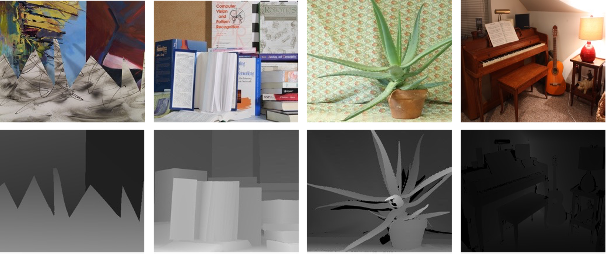
\includegraphics{figures/27.png}
	\caption{Middlebury 数据集彩色图像和深度图像示例}
	\label{fig:fig4-1}
	\vspace{-0.8cm}  %调整图片与下文的垂直距离
\end{figure}

\newpage
\item[(2)] NUY v2 \newline
NYU v2 的原始数据集包含了464个室内场景,是由 RGB-D 摄像机获取的场景的单目视频序列和对应的深度真值。其中,1449个图像对被标注了密集标签且已经对缺失值进行了填充,可以直接用于深度图像超分辨率重建任务。这些带有标签的图像分辨率为 $640 \times 480$,部分彩色图像和对应的深度图像如图 \ref{fig:fig4-2} 所示。

	\begin{figure}[!htbp]
%	\vspace{-0.8cm}  %调整图片与上文的垂直距离
	\centering
	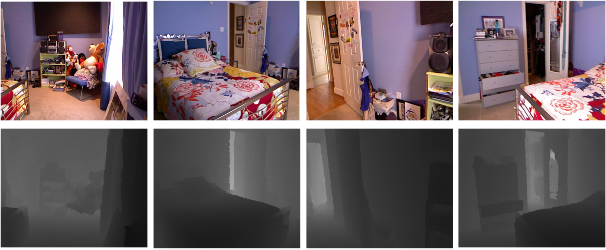
\includegraphics{figures/28.png}
	\caption{NYU v2 数据集彩色图像和深度图像示例}
	\label{fig:fig4-2}
	\vspace{-0.8cm}  %调整图片与下文的垂直距离
	\end{figure}
	
\end{itemize}

\subsection{评价指标}

本文选择了平均绝对差(Mean Absolute Difference, MAD)和均方根误差(Root Mean Square Error, RMSE)来度量超分辨率重建得到的深度图像与真值之间的差异。

对于 Middlebury 数据集 $X=\{I_{HR}^n,D_{HR}^n,D_{LR}^n\}_{n=1}^N$, $I_{HR}^n,D_{HR}^n,D_{LR}^n$ 分别为高分辨率彩色图像和深度图像以及对应的低分辨率深度图像,$N$ 为数据集中图像的数量,则平均绝对差可以定义为式 \ref{equ:equ4-1}。

\begin{equation}
	MAD_{Middlebury}=\frac{1}{N}\sum_{n=1}^{N}\left|D_{HR}^n-SR\left(D_{LR}^n\right)\right|
	\label{equ:equ4-1}
\end{equation}

\noindent 式中,$SR$ —— 超分辨率重建操作。

同样,对于 NYU v2 数据集 $Y=\{I_{HR}^m,D_{HR}^m,D_{LR}^m\}_{m=1}^M$, $I_{HR}^m,D_{HR}^m,D_{LR}^m$ 分别为高分辨率彩色图像和深度图像以及对应的低分辨率深度图像,$M$ 为数据集中图像的数量,则均方根误差可以定义为式 \ref{equ:equ4-2}。

\begin{equation}
	{RMSE}_{NYU\ v2}=\sqrt{\frac{1}{M}\sum_{m=1}^{M}\left(D_{HR}^m-SR\left(D_{LR}^m\right)\right)^2}
	\label{equ:equ4-2}
\end{equation}

\noindent 式中,$SR$ —— 超分辨率重建操作。

\section{实验配置}

本文从 Middlebury 数据集中收集了36对 RGB-D 图像对(分别来自2001 \cite{DBLP:journals/ijcv/BakerSLRBS11},2006 \cite{DBLP:conf/cvpr/HirschmullerS07} 和2014 \cite{DBLP:conf/dagm/ScharsteinHKKNWW14} 的6、21、9张图像)用于训练,将 Middlebury 2005 \cite{DBLP:conf/cvpr/ScharsteinP07} 数据集中的6对 RGB-D 对图像对(分别为 Art,Books,Moebius,Dolls,Laundry,Reindeer)用于测试。本文选取的另一个用于训练和测试的数据集是 NYU v2 数据集 \cite{SilbermanHKF12},并按照通用的划分方法 \cite{DBLP:conf/eccv/LiHA016},将数据集中的前 1000 对 RGB-D 图像对作为训练数据,然后在后449对 RGB-D 图像对上进行评估。此外,用于训练和测试的 RGB-D 图像对被归一在 [0,1] 范围内。

遵循现有工作的方法[10],本文在高分辨率图像输入网络前将其划分为具有重叠的规则网格,即把一幅完整的图像裁剪成足够数量的图像块。这种训练策略不仅不会削弱网络的性能,而且会减少训练的时间。高分辨率的深度图像和彩色图像分别根据 $\times 4$、$\times 8$ 和 $\times 16$ 的上采样因子被裁剪成足够数量(在本文实验中一般裁剪为15000张左右的图像块)的大小为 ${64}^2$、${128}^2$ 和 ${256}^2$ 的图像块。为了获得相应的低分辨率深度图像块,本文使用 Bicubic 插值方法将高分辨率深度图像块下采样为固定大小的 $16 \times 16$ 的图像块。如前文所述,本文引入了平均绝对差(MAD)和均方根误差(RMSE)两个指标,以对模型的性能进行定量评估。

本文提出的网络基于深度学习框架 PyTorch 实现,并使用 NVIDIA 2080Ti GPU 加速训练。在训练期间,一次训练所选取的样本数(Batch Size)为 8。此外,本文选取了动量为 0.9,$\beta_1=0.9$,$\beta_2=0.99$,$\epsilon={10}^{-8}$ 的 ADAM 优化器对训练进行优化。初始学习率设置为 $1e^{-4}$,并且每100轮(epoch)乘以0.1以降低学习速率。在上采样因子为 $\times 8$ 的深度图像超分辨率重建实验中,大小为 $256 \times 256$ 的图像的推理时间为0.052 秒。

\section{基于 Middlebury 数据集的结果比较及分析}

本文在不同上采样因子($\times 4$,$\times 8$ 和 $\times 16$)与一些最新的深度图像超分辨率重建方法进行了比较,包括六种传统深度图像超分辨率重建算法(即 CLMF \cite{LuSMLD12},JGF \cite{0001TT13},TGV \cite{DBLP:conf/iccv/FerstlRRRB13},CDLLC \cite{DBLP:conf/icmcs/XieCFS14},PB \cite{DBLP:conf/eccv/AodhaCNB12} 和 EG \cite{DBLP:journals/tip/XieFS16})和七种基于深度学习的方法(即 SRCNN \cite{DBLP:conf/eccv/DongLHT14}, ATGVNet \cite{DBLP:conf/eccv/RieglerRB16}, MSG \cite{HuiLT16}, DGDIE \cite{DBLP:conf/cvpr/GuZGCCZ17}, DEIN \cite{DBLP:conf/icassp/YeDL18}, CCFN \cite{WenSLLF19}, GSRPT \cite{LutioDWS19}, 和 CTKT \cite{Sun2021cvpr})。

图 \ref{fig:fig4-3} 展示了 $\times 8$ 上采样因子下不同方法在图像 Art 和 Dolls 上的可视化结果比较。其中,(a)为深度图像的真值(Ground Truth)和彩色图像;(b)为低分辨率深度块;(c)-(h)分别为通过 Bicubic,TGV \cite{DBLP:conf/iccv/FerstlRRRB13},MSG \cite{HuiLT16},CTKT \cite{Sun2021cvpr} 和 BridgeNet 超分辨率重建得到的深度图像块;(i)为深度图像的真值图像块。为了获得更加清晰的可视化结果,深度图像块经过了放大。

\newpage
显然,就场景的结构和细节而言,与深度图像的真值相比,本文的方法获得了最相似的重建结果。对于图中的尺寸较大的物体(如 Art 中的茶壶),所有的基于深度学习的方法都呈现出相似的重建结果。然而,对于微小的物体,本文的方法可以恢复深度图像更多的细节。例如,Art 图像中的棍子周围的伪影更少,Doll 图像中的玩具头部轮廓更准确。而其他方法可能会产生一些伪像,边界模糊或形状变化。这些现象与低分辨率深度图像成像时深度相机对精细结构和微小物体的严重破坏有关,从而给这些区域的重建带来了更多困难。因此,本文的方法在准确恢复这些微小物体的深度边界方面更具有优势。

\begin{figure}[!htbp]
%	\vspace{-0.8cm}  %调整图片与上文的垂直距离
	\centering
	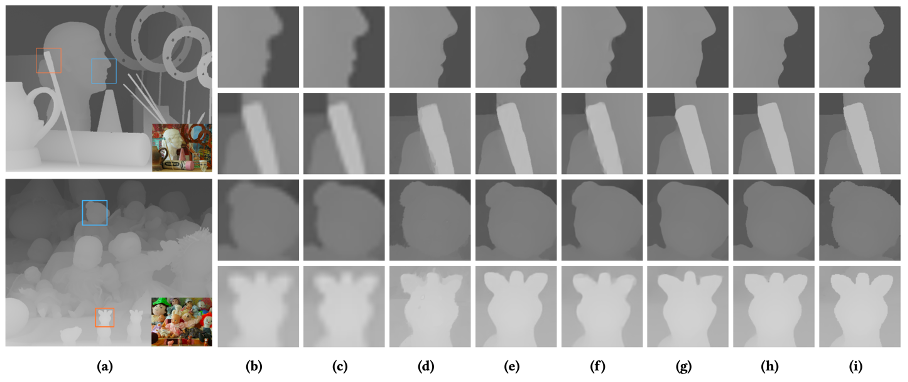
\includegraphics{figures/29.png}
	\caption{Middlebury 数据集 $\times 8$ 不同超分辨率重建方法可视化结果对比}
	\label{fig:fig4-3}
	\vspace{-0.8cm}  %调整图片与下文的垂直距离
	\end{figure}
	
	与其他方法的定量比较如表 \ref{tab:tab4-1} 和表 \ref{tab:tab4-2} 所示(性能最好的模型指标被加粗显示,而性能排名第二的模型指标被下划线标记)。与基于卷积神经网络的方法相比,传统的基于滤波或基于优化的方法具有相对较高的平均绝对差值。而与其他基于卷积神经网络的方法相比,本文提出的单目深度估计和深度图像超分辨率重建联合学习网络(BridgeNet)可以获得具有竞争力的结果,即使在 $\times 8$ 和 $\times 16$ 这样具有挑战性的上采样因子下,本文提出的网络也几乎可以获得最佳的结果。以上采样因子为 $\times 16$ 的深度图像超分辨率重建实验为例,对于 Books 图像,与性能排名第二的算法相比,本文的方法将 MAD 从0.67提升至0.51,百分比增益为23.9%。
	
%\renewcommand{\arraystretch}{0.85}
\setlength{\tabcolsep}{3.5mm}{
\begin{longtable}{c|ccc|ccc|ccc}
\caption{Middlebury 数据集 $\times 8$ 不同超分辨率重建方法量化指标对比(一)}
\label{tab:tab4-1}\\
\toprule[1.5pt]
\multirow{2}{*}{} & \multicolumn{3}{c|}{Art} & \multicolumn{3}{c|}{Books} & \multicolumn{3}{c}{Dolls} \\\cline{2-10}
                  &  $\times 4$      &  $\times 8$      &   $\times 16$    &   $\times 4$      &     $\times 8$   &    $\times 16$    &    $\times 4$     &    $\times 8$    &    $\times 16$    \\\hline
\endfirsthead
\multicolumn{10}{c}%
{\hfill{\zihao{5} 表 \thetable\ (续)}} \\
\toprule[1.5pt]
\multirow{2}{*}{} & \multicolumn{3}{c|}{Art} & \multicolumn{3}{c|}{Books} & \multicolumn{3}{c}{Dolls} \\\cline{2-10}
                  &  $\times 4$      &  $\times 8$      &   $\times 16$    &   $\times 4$      &     $\times 8$   &    $\times 16$    &    $\times 4$     &    $\times 8$    &    $\times 16$    \\\hline
\endhead

CLMF \cite{LuSMLD12}       & 0.76 & 1.44 & 2.87       & 0.28    & 0.51   & 1.02   & 0.34    & 0.60   & 1.01   \\
JGF \cite{0001TT13}        & 0.47 & 0.78 & 1.54       & 0.24    & 0.43   & 0.81   & 0.33    & 0.59   & 1.06   \\
TGV \cite{DBLP:conf/iccv/FerstlRRRB13}        & 0.65 & 1.17 & 2.30       & 0.27    & 0.43   & 0.82   & 0.33    & 0.70   & 2.20   \\
CDLLC \cite{DBLP:conf/icmcs/XieCFS14}     & 0.53 & 0.76 & 1.41       & 0.19    & 0.46   & 0.75   & 0.31    & 0.53   & 0.79   \\\bottomrule[1.5pt]
PB \cite{DBLP:conf/eccv/AodhaCNB12}        & 0.79 & 0.93 & 1.98       & 0.16    & 0.43   & 0.79   & 0.53    & 0.83   & 0.99   \\
EG \cite{DBLP:journals/tip/XieFS16}        & 0.48 & 0.71 & \uline{1.35}     & 0.15    & 0.36   & 0.70   & 0.27    & 0.49   & 0.74  \\\hline
SRCNN \cite{DBLP:conf/eccv/DongLHT14}     & 0.63          & 1.21          & 2.34          & 0.25          & 0.52          & 0.97          & 0.29          & 0.58          & 1.03          \\
ATGVNet \cite{DBLP:conf/eccv/RieglerRB16}   & 0.65          & 0.81          & 1.42          & 0.43          & 0.51          & 0.79          & 0.41          & 0.52          & \textbf{0.56} \\
MSG \cite{HuiLT16}       & 0.46          & 0.76          & 1.53          & 0.15          & 0.41          & 0.76          & 0.25          & 0.51          & 0.87          \\
DGDIE \cite{DBLP:conf/cvpr/GuZGCCZ17}    & 0.48          & 1.20          & 2.44          & 0.30          & 0.58          & 1.02          & 0.34          & 0.63          & 0.93          \\
DEIN \cite{DBLP:conf/icassp/YeDL18}        & 0.40          & 0.64          & \textbf{1.34} & 0.22          & 0.37          & 0.78          & 0.22          & 0.38          & 0.73          \\
CCFN \cite{WenSLLF19}    & 0.43          & 0.72          & 1.50          & 0.17          & 0.36          & 0.69          & 0.25          & 0.46          & 0.75          \\
GSRPT \cite{LutioDWS19}     & 0.48          & 0.74          & 1.48          & 0.21          & 0.38          & 0.76          & 0.28          & 0.48          & 0.79          \\
CTKT \cite{Sun2021cvpr}      & \textbf{0.25} & \textbf{0.53} & 1.44          & \textbf{0.11} & \uline{0.26}    & \uline{0.67}    & \textbf{0.16} & \uline{0.36}    & 0.65          \\
BridgeNet         & \uline{0.30}    & \uline{0.58}    & 1.49          & \uline{0.14}    & \textbf{0.24} & \textbf{0.51} & \uline{0.19}    & \textbf{0.34} & \uline{0.64}   \\
\bottomrule[1.5pt]
\end{longtable}}

\setlength{\tabcolsep}{3.5mm}{
\begin{longtable}{c|ccc|ccc|ccc}
\caption{Middlebury 数据集 $\times 8$ 不同超分辨率重建方法量化指标对比(二)}
\label{tab:tab4-2}\\
\toprule[1.5pt]
\multirow{2}{*}{} & \multicolumn{3}{c|}{Art} & \multicolumn{3}{c|}{Books} & \multicolumn{3}{c}{Dolls} \\\cline{2-10}
                  &  $\times 4$      &  $\times 8$      &   $\times 16$    &   $\times 4$      &     $\times 8$   &    $\times 16$    &    $\times 4$     &    $\times 8$    &    $\times 16$    \\\hline
\endfirsthead
\multicolumn{10}{c}%
{\hfill{\zihao{5} 表 \thetable\ (续)}} \\
\toprule[1.5pt]
\multirow{2}{*}{} & \multicolumn{3}{c|}{Art} & \multicolumn{3}{c|}{Books} & \multicolumn{3}{c}{Dolls} \\\cline{2-10}
                  &  $\times 4$      &  $\times 8$      &   $\times 16$    &   $\times 4$      &     $\times 8$   &    $\times 16$    &    $\times 4$     &    $\times 8$    &    $\times 16$    \\\hline
\endhead

CLMF \cite{LuSMLD12}     & 0.50 & 0.80       & 1.67          & 0.29 & 0.51 & 0.97 & 0.51 & 0.84 & 1.55          \\ 
JGF \cite{0001TT13}      & 0.36 & 0.64       & 1.20          & 0.25 & 0.46 & 0.80 & 0.38 & 0.64 & 1.09          \\ 
TGV \cite{DBLP:conf/iccv/FerstlRRRB13}      & 0.55 & 1.22       & 3.37          & 0.29 & 0.49 & 0.90 & 0.49 & 1.03 & 3.05          \\ 
CDLLC \cite{DBLP:conf/icmcs/XieCFS14}   & 0.30 & 0.48       & 0.96          & 0.27 & 0.46 & 0.79 & 0.43 & 0.55 & 0.98          \\ 
PB \cite{DBLP:conf/eccv/AodhaCNB12}      & 1.13 & 1.89       & 2.87          & 0.17 & 0.47 & 0.82 & 0.56 & 0.97 & 1.89          \\ 
EG \cite{DBLP:journals/tip/XieFS16}      & 0.28 & 0.45       & \uline{0.92}    & 0.23 & 0.42 & 0.75 & 0.36 & 0.51 & 0.95          \\ \hline
SRCNN \cite{DBLP:conf/eccv/DongLHT14}   & 0.40 & 0.87       & 1.74          & 0.25 & 0.43 & 0.87 & 0.35 & 0.75 & 1.47          \\
ATGVNet \cite{DBLP:conf/eccv/RieglerRB16} & 0.37 & 0.89       & 0.94          & 0.38 & 0.45 & 0.80 & 0.41 & 0.58 & 1.01 \\
MSG \cite{HuiLT16}    & 0.30 & 0.46       & 1.12          & 0.21 & 0.43 & 0.76 & 0.31 & 0.52 & 0.99          \\
DGDIE \cite{DBLP:conf/cvpr/GuZGCCZ17}   & 0.35 & 0.86       & 1.56          & 0.28 & 0.58 & 0.98 & 0.35 & 0.73 & 1.29          \\
DEIN \cite{DBLP:conf/icassp/YeDL18}      & 0.23 & \uline{0.36} & 0.81 & 0.20 & 0.35 & 0.73 & 0.26 & 0.40 & 0.80          \\
CCFN \cite{WenSLLF19}   & 0.24 & 0.41       & 0.71          & 0.23 & 0.39 & 0.73 & 0.29 & 0.46 & 0.95          \\
GSRPT \cite{LutioDWS19}   & 0.33 & 0.56       & 1.24          & 0.24 & 0.49 & 0.80 & 0.31 & 0.61 & 1.07          \\
CTKT \cite{Sun2021cvpr}      & \textbf{0.16} & \uline{0.36}    & \uline{0.76}    & \textbf{0.13} & \uline{0.27}    & \uline{0.69}    & \textbf{0.17} & \uline{0.35}    & \uline{0.77}          \\
BridgeNet         & \uline{0.17}    & \textbf{0.34} & \textbf{0.71} & \uline{0.15}    & \textbf{0.26} & \textbf{0.54} & \uline{0.19}    & \textbf{0.31} &  \textbf{0.70}\\
\bottomrule[1.5pt]
\end{longtable}}

\section{基于 NYU v2 数据集的结果比较及分析}

本文还在 NYU v2 数据集上对提出的方法进行评估,并与其他最新的方法进行比较,包括 Bicubic,TGV \cite{DBLP:conf/iccv/FerstlRRRB13}, EDGE \cite{ParkKTBK11}, DJF \cite{DBLP:conf/eccv/LiHA016}, SDF \cite{DBLP:journals/pami/HamCP18}, DGDIE \cite{DBLP:conf/cvpr/GuZGCCZ17}, GbFT \cite{DBLP:conf/iccv/AlbaharH19}, PAC \cite{DBLP:conf/cvpr/SuJSGLK19}, SVLRM \cite{DBLP:conf/cvpr/PanDRLT019}, DKN \cite{DBLP:journals/corr/abs-1903-11286} 和 CTKT \cite{Sun2021cvpr}。

图 \ref{fig:fig4-4} 展示了本文的方法在 $\times 8$ 上采样因子下的可视化结果。其中,(a)为彩色图像;(b)为深度图像真值;(c)-(f)分别为SDF  \cite{DBLP:journals/pami/HamCP18},DJF  \cite{DBLP:conf/eccv/LiHA016},SVLRM  \cite{DBLP:conf/cvpr/PanDRLT019} 和 BridgeNet 超分辨率重建得到的深度图像块。可以看到,无论是在红色矩形区域还是在黄色矩形区域内,本文的方法都可以准确地重建图像的深度信息和微小物体的边缘。如表 \ref{tab:tab4-3} 中所示(性能最好的模型指标被加粗显示,而性能排名第二的模型指标被下划线标记),在 $\times 8$ 和 $\times 16$ 上采样因子的情况下,本文的方法可以获得最佳的性能。与性能排名第二的算法相比,本文方法的 RMSE 在 $\times 8$ 的上采样因子下达到2.63,提升了3.7%。

\begin{figure}[!htbp]
%	\vspace{-0.8cm}  %调整图片与上文的垂直距离
	\centering
	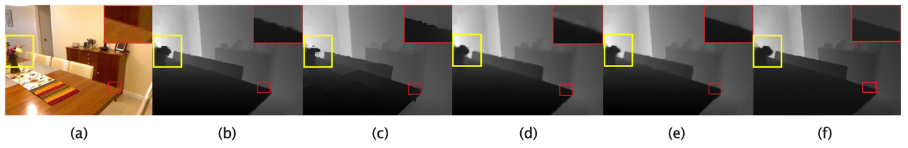
\includegraphics{figures/30.png}
	\caption{NYU v2 数据集 $\times 8$ 不同超分辨率重建方法可视化结果对比}
	\label{fig:fig4-4}
	\vspace{-0.8cm}  %调整图片与下文的垂直距离
	\end{figure}
	
\setlength{\tabcolsep}{14mm}{	
\begin{longtable}{c|ccc}
\caption{NYU v2 数据集 \textbackslash{}times8 不同超分辨率重建方法量化指标对比}
\label{tab:tab4-3}\\
\toprule[1.5pt]
               &     $\times 4$          &         $\times 8$      &        $\times 16$     \\\hline
\endfirsthead
%
\multicolumn{4}{c}%
{\hfill{\zihao{5} 表 \thetable\ (续)}} \\
\toprule[1.5pt]
              &     $\times 4$          &         $\times 8$      &        $\times 16$       \\\hline
\endhead
%
Bicubic       & 8.16          & 14.22         & 22.32         \\
TGV \cite{DBLP:conf/iccv/FerstlRRRB13}    & 6.98          & 11.23         & 28.13         \\
EDGE \cite{ParkKTBK11}   & 5.21          & 9.56          & 18.1          \\
DJF \cite{DBLP:conf/eccv/LiHA016}   & 3.54          & 6.2           & 10.21         \\
SDF \cite{DBLP:journals/pami/HamCP18}   & 3.04          & 5.67          & 9.97          \\
DGDIE \cite{DBLP:conf/cvpr/GuZGCCZ17} & 1.56          & 2.99          & 5.24          \\
GbFT \cite{DBLP:conf/iccv/AlbaharH19}  & 3.35          & 5.73          & 9.01          \\
PAC \cite{DBLP:conf/cvpr/SuJSGLK19}   & 2.39          & 4.59          & 8.09          \\
SVLRM \cite{DBLP:conf/cvpr/PanDRLT019} & 1.74          & 5.59          & 7.23          \\
DKN \cite{DBLP:journals/corr/abs-1903-11286}   & 1.62          & 3.26          & 6.51          \\
CTKT \cite{Sun2021cvpr}  & \textbf{1.49} & \uline{2.73}    & \uline{5.11}    \\
BridgeNet     & \uline{1.54}    & \textbf{2.63} & \textbf{4.98}\\
\bottomrule[1.5pt]
\end{longtable}}
	
\section{消融实验}
在本节中,将进行全面的消融研究以验证单目深度估计和深度图像超分辨率重建联合学习网络(BridgeNet)中的设计对提升深度图像超分辨率重建性能的作用及贡献。表 \ref{tab:tab4-4} 列出了 Middlebury 2005数据集在不同实验设计下进行八倍上采样深度图像超分辨率重建的结果。第一行和第二行是在相同条件下分别单独对深度图像超分辨率重建子网络和单目深度估计子网络训练与测试的结果。从平均绝对差的值来看,单目深度估计子网络的性能不及深度图像超分辨率重建子网络,这样的结果与之前的分析吻合。也就是说,单目深度估计任务的学习难度与深度图像超分辨率重建任务相比较为困难。

对于任务间的交互,本文首先通过简单的损失函数约束将两个任务组合在一起,结果为表 \ref{tab:tab4-4} 的第三行。与单独的深度图像超分辨率重建子网络相比,深度图像超分辨率重建的 MAD 优化到0.363。然后,逐渐将高频注意力桥(HABdg)和内容引导桥(CGBdg)集成到网络中以验证它们的作用。在联合学习网络中仅使用高频注意力桥或内容引导桥时,获得的结果要好于仅使用损失函数约束。此外,当两个桥接器一起工作时(即完整模型),网络的性能将达到最佳。本文还在图 \ref{fig:fig4-5} 中提供了一些可视化的比较,其中(a)为深度图像真值;(b)为单独的深度图像超分辨率重建子网络(DSRNet)的结果;(c)为 BridgeNet 的结果。从图中可以看出,与单独的深度图像超分辨率重建子网络相比,本文的模型具有更清晰的边界和更准确的深度值,如图中的黄色矩形区域所示。

\begin{table}[!ht]

%\setlength{\abovecaptionskip}{0.2cm}
%\setlength{\belowcaptionskip}{-0.1cm}

\renewcommand\arraystretch{1}
\caption{针对 BridgeNet 的消融研究量化对比}
\centering
\label{tab:tab4-4}
\setlength{\tabcolsep}{7mm}{
\begin{tabular}{c|cccc|c}
%\hline
\toprule[1.5pt]
& DSRNet & MDENet & HABdg & CGBdg & Middlebury\\
\hline
1 &\checkmark & & &  & 0.366\\
2& & \checkmark &  & & 0.472\\
 \hline
3&\checkmark & \checkmark  & & & 0.363\\
4&\checkmark & \checkmark  &\checkmark & & 0.355\\
5&\checkmark & \checkmark  &  & \checkmark & 0.361\\
\hline
6&\checkmark & \checkmark & \checkmark & \checkmark & 0.343\\
\bottomrule[1.5pt]
\end{tabular}}
\end{table}

\begin{figure}[!htbp]
%	\vspace{-0.8cm}  %调整图片与上文的垂直距离
	\centering
	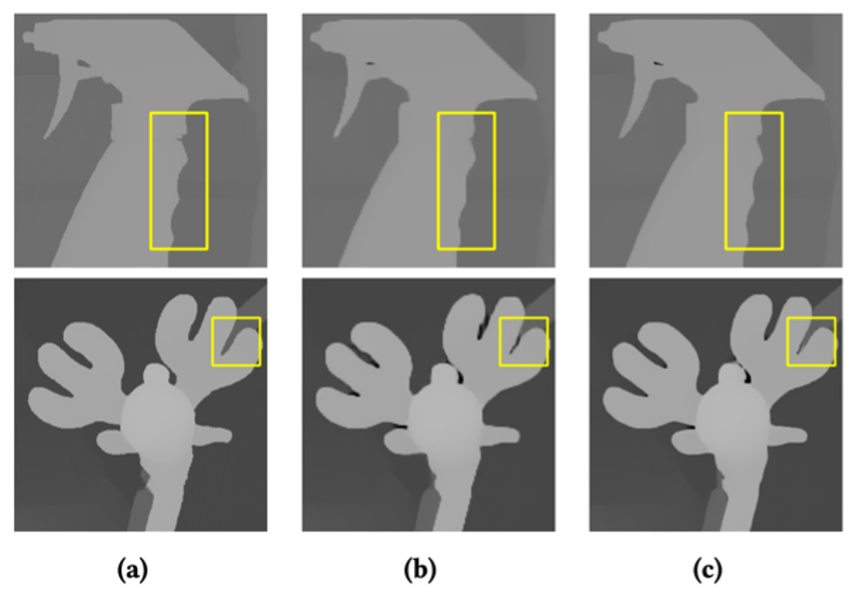
\includegraphics{figures/31.png}
	\caption{消融实验可视化结果对比}
	\label{fig:fig4-5}
	\vspace{-0.8cm}  %调整图片与下文的垂直距离
	\end{figure}

为了进一步证明高频注意力桥的有效性,本文通过将单目深度估计子网络的特征未经任何处理地馈入到深度图像超分辨率重建子网络来代替它,并在 Middlebury 数据集上进行了训练,以及在 Middlebury 2005数据集上进行了上采样因子为 $\times 8$ 的对比实验,量化指标结果如表 \ref{tab:tab4-5} 所示(w/o HABdg 指的是通过直接将单目深度估计子网络的特征传递给深度图像超分辨率重建子网络代替高频注意力桥)。与简单地将通道维度上的特征级联并送入深度图像超分辨率重建网络相比,本文提出的高频注意力桥可以提供更有效的高频指导以提高性能。

\begin{table}[]
\caption{针对高频注意力桥的消融研究量化对比}
\label{tab:tab4-5}
\setlength{\tabcolsep}{3.7mm}{
\begin{tabular}{c|cccccc|c}
\toprule[1.5pt]
          & Art  & Books & Dolls & Laundry & Mobius & Reindeer & Avg.  \\\hline
w/ HABdg  & 0.58 & 0.24  & 0.34  & 0.34    & 0.26   & 0.31     & 0.343 \\
w/o HABdg & 0.65 & 0.25  & 0.37  & 0.38    & 0.28   & 0.33     & 0.376 \\
\bottomrule[1.5pt]
\end{tabular}}
\end{table}

\section{本章小结}

本章主要介绍了本文所设计的实验及其测试结果,包括在不同数据集上与最新方法的可视化对比和评价指标的比较。首先,介绍了本文采用的公开基准数据集和评估指标,并对有关实验的详细配置进行了阐明,然后介绍了本文提出的单目深度估计和深度图像超分辨率重建联合学习网络在 Middlebury 数据集上不同上采样因子的实验结果及分析,并与最新的深度超分辨率重建算法的结果进行了对比。同样,本文也将 NYU v2 数据集上不同上采样因子的实验结果与代表性的方法进行了对比和分析。此外,本文通过设计详尽的消融实验探究了所提出网络设计的有效性,验证了两个桥接器对提升深度图像超分辨率重建任务性能的积极作用。
